%
% Documento: Fundamentação Teórica
%

\chapter{Fundamentação Teórica}
\label{chap:fundamentacaoTeorica}

Este capítulo apresenta os principais conceitos relacionados ao funcionamento e à utilização do protocolo HTTP, bem como traça comparações entre suas versões. O bom entendimento do funcionamento do protocolo, bem como do uso que é feito dele na \textit{web}, é essencial para a compreensão das técnicas de otimização de desempenho que serão apresentadas e avaliadas neste trabalho.

\section{O Protocolo HTTP}
\label{sec:http}

Nas década de 1970 e 1980 a comunidade cientifica estava trabalhando arduamente para fazer importantes descobertas. O problema é que por causa das distâncias geográficas era muito difícil de compartilhar informações e isso atrasava os tão esperados avanços da ciência. Apesar dos avanços na área de rede de computadores, essas não conseguiam resolver o problema dos cientistas. Existiam várias redes espalhadas pelos Estados Unidos e Europa, mas como cada uma possuía topologia e sistemas operacionais diferentes elas não se comunicavam entre si, limitando a troca de informação aos computadores conectados na mesma rede. Visando resolver esse problema em 1989, o cientista do CERN \footnote{Organização Europeia para Pesquisa Nuclear, conhecida como CERN na sigla em inglês, é uma organização de pesquisas em física e engenharia que realiza experimentos para tentar compreender as estruturas fundamentais do universo.}, Tim Berners-Lee, propôs uma rede de computadores global para ajudar a comunidade científica a compartilhar o conhecimento gerado em diferentes partes do mundo, acelerando assim o desenvolvimento tecnológico. Para isso Tim precisaria de um formato padrão de arquivos que pudesse ser executado em qualquer computador, assim desenvolveu uma linguagem de marcação de hipertextos,  que ficou conhecida como HTML, e um programa para executar esses arquivos, um navegador \textit{web}. Esses arquivos precisariam ser servidos sempre que fossem requisitados, então Berners-Lee criou um servidor \textit{web}. E por último era necessário um protocolo para conectar o navegador ao servidor, então foi desenvolvido o protocolo para transferência de hipertextos, chamado de HTTP. Ao final de 1990, Tim Berners-Lee já havia terminado de desenvolver todos os requisitos necessários para sua rede, e decidiu chamá-la de \textit{World Wide Web}, hoje conhecida apenas como \textit{web}.

O protocolo HTTP baseava-se na troca de informações por meio de mensagens formadas por caracteres ASCII, ou seja, mensagens de texto. O navegador \textit{web} enviava uma requisição, como a exemplificada na \autoref{fig:exemplorequisicaohttp}, e o servidor retornava uma resposta, como a da \autoref{fig:exemplorespostahttp}. O protocolo era simples.

\begin{figure}[!htb]
    \centering
    \caption{Exemplo de requisição HTTP}
    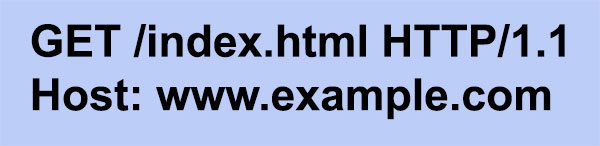
\includegraphics[width=0.3\textwidth]{./04-figuras/fund-teorica/http_exemplo_requisicao}
    \label{fig:exemplorequisicaohttp}
\end{figure}

\begin{figure}[!htb]
    \centering
    \caption{Exemplo de resposta HTTP}
    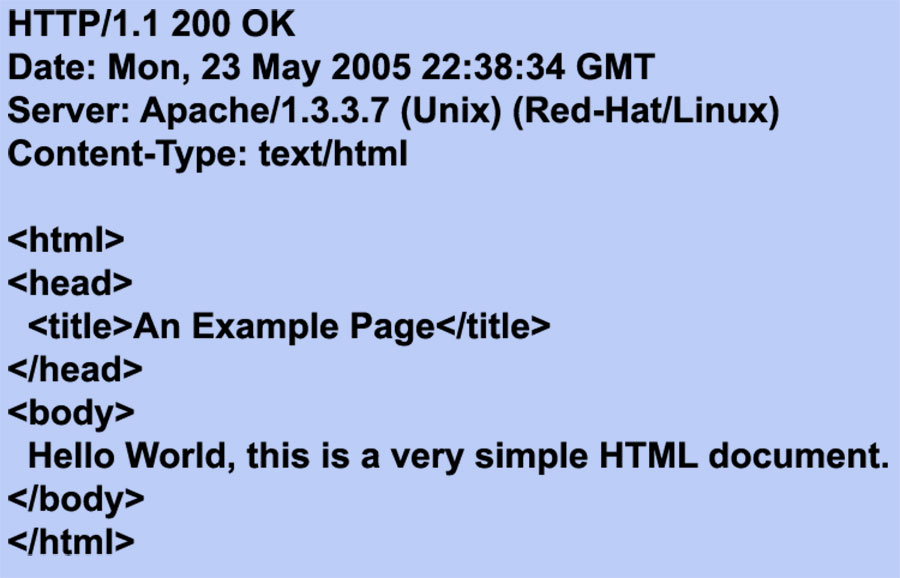
\includegraphics[width=0.4\textwidth]{./04-figuras/fund-teorica/http_exemplo_resposta}
    \label{fig:exemplorespostahttp}
\end{figure}

Apesar de ter sido utilizado desde 1990, o HTTP recebeu sua primeira documentação oficial em 1991, quando recebeu um número de versão e passou a ser chamado de HTTP/0.9. A ideia é explicada por \citeonline{HighPerformanceBrowserNetworking} da seguinte maneira:

\begin{itemize}
	\item Uma conexão TCP era aberta entre o navegador (chamado também de cliente) e o servidor
	\item A requisição do cliente era uma cadeia simples de caracteres ASCII
	\item A resposta do servidor era uma torrente de caracteres ASCII que representava um arquivo HTML
	\item A conexão era fechada após a transferência do documento 
\end{itemize}

Com o passar dos anos, a \textit{World Wide Web} de Tim Berners-Lee cresceu rapidamente e isso fez com que o uso do HTTP aumentasse muito em pouco tempo. Viu-se a necessidade de um protocolo mais robusto e estruturado, mas que mantivesse a simplicidade do HTTP/0.9, pois esta era vista como o motivo por trás do sucesso do protocolo. Então o IETF \footnote{Força Tarefa de Engenharia da Internet, conhecida como IETF na sigla em inglês, é uma comunidade aberta formada por profissionais que se preocupam com a evolução da Internet e por isso procuram formalizar as técnicas utilizadas na rede global de computadores.} passou a coordenar a criação de especificações para o HTTP e criou o HTTP-WG \footnote{Grupo de Trabalho do HTTP, conhecido como HTTP-WG na sigla em inglês, é um grupo formado por profissionais escolhidos pelo IETF} que tinha a função definir as especificações das versões seguintes do protocolo. Em 1996 foi definido o HTTP/1.0 \cite{RFC1945}, em 1999 o HTTP/1.1 \cite{RFC2616} e em 2015 foi aprovada a especificação para o HTTP2 \cite{HTTP2Spec}.

\section{Visão Geral}
\label{sec:http_visão_geral}

Como descrito por \citeonline[p.~683]{Tanenbaum}, o HTTP é um simples protocolo de requisições e respostas. As requisições e respostas são compostas por um cabeçalho e um conteúdo, e são enviadas do cliente para o servidor. O HTTP é um protocolo independente de estado, ou seja, cada tupla requisição-resposta pode ser tratada de maneira independente, sem que as anteriores e futuras interfiram nela. O modelo, ilustrado na \autoref{fig:httpoverview}, é bem simples e direto, fácil de ser replicado.

\begin{figure}[!htb]
    \centering
    \caption{Visão Geral do Protocolo HTTP}
    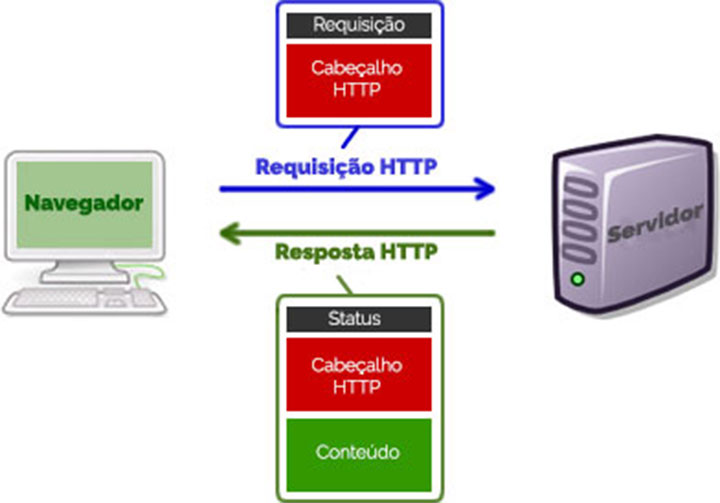
\includegraphics[width=0.6\textwidth]{./04-figuras/fund-teorica/http_overview}
    \fonte{Adaptado de \citeonline{ImagemHTTPOverview}}
    \label{fig:httpoverview}
\end{figure}

O HTTP foi desenvolvido para funcionar na camada de Aplicação do protocolo TCP, conectando as ações do usuário à camada de Apresentação. Contudo, de acordo com \citeonline[p.~684]{Tanenbaum}, ele se transformou em um protocolo da camada de Transporte, criando uma maneira de processos se comunicarem através de diferentes redes. Hoje em dia não são apenas os navegadores \textit{web} que utilizam o protocolo HTTP para se comunicar com servidores, aplicações como tocadores de mídias, anti-vírus, programas de fotos, dentre outras utilizam o HTTP para trocar informações de maneira simples, rápida e eficiente.

Os cabeçalhos HTTP definem características desejadas ou esperadas pelas aplicações e servidores, como tipo de codificação de caracteres ou tipo de compressão dos dados. Existem várias etiquetas padrões que podem ser utilizadas nos cabeçalhos e os desenvolvedores podem ainda criar etiquetas próprias para serem utilizadas dentro das aplicações - por definição, caso um cliente ou servidor receba uma etiqueta que não reconhece ele simplesmente a ignora. No \autoref{qua:cabecalhoshttp} são apresentadas algumas das etiquetas mais utilizadas, mas existem muitas outras que não foram citadas e que podem variar com a versão do protocolo.

\begin{quadro}[!htb]
	\centering
	\caption{Etiquetas para cabeçalhos HTTP.\label{qua:cabecalhoshttp}}
	\begin{tabular}{| c | c | c |}
		\hline
		\textbf{Etiqueta} & \textbf{Tipo} & \textbf{Conteúdo}                                       \\
		\hline
		\textit{Accept}             & Requisição    & Tipo de páginas que o cliente suporta                   \\
		\hline
		\textit{Accept-Encoding}    & Requisição    & Tipo de codificação que o cliente suporta               \\
		\hline
		\textit{If-Modified-Since}  & Requisição    & Data e hora para checar atualidade do conteúdo          \\
		\hline
		\textit{Authorization}      & Requisição    & Uma lista de credenciais do cliente                      \\
		\hline
		\textit{Cookie}             & Requisição    & Cookie definido previamente enviado para o servidor     \\
		\hline
		\textit{Content-Encoding}   & Resposta      & Como o conteúdo foi codificado (e.g. \textit{gzip})               \\
		\hline
		\textit{Content-Length}     & Resposta      & Tamanho da página em \textit{bytes}                              \\
		\hline
		\textit{Content-Type}       & Resposta      & Tipo de \textit{MIME} da página                                  \\
		\hline
		\textit{Last-Modified}      & Resposta      & Data e hora que a página foi modificada pela última vez \\
		\hline
		\textit{Expires}            & Resposta      & Data e hora quando a página deixa de ser válida         \\
		\hline
		\textit{Cache-Control}      & Ambas          & Diretiva de como tratar \textit{cache}                           \\
		\hline
		\textit{ETag}               & Ambas          & Etiqueta para o conteúdo da página                      \\
		\hline
		\textit{Upgrade}            & Ambas          & O novo protocolo para o qual o cliente deseja alterar        \\	
		\hline
	\end{tabular}
	\fonte{Adaptado de \citeonline{Tanenbaum}}
\end{quadro}

O conteúdo de uma resposta HTTP pode assumir diferentes formatos (como, HTML, CSS e JavaScript) e a definição desse formato é feita com a etiqueta \textit{Content-Type} enviada no cabeçalho de resposta. O conteúdo é a maior parte de uma resposta HTTP e os desenvolvedores devem se esforçar para reduzi-lo ao máximo, garantindo que a comunicação de dados seja rápida e eficiente.

Por executar em cima do protocolo TCP, o HTTP precisa que uma conexão TCP seja aberta para poder realizar a troca de dados entre o cliente e o servidor. Como essa conexão é gerenciada depende da versão do protocolo. Após a abertura da conexão, a requisição pode ser enviada. Na primeira linha da requisição, são definidas a versão do protocolo e a operação que será realizada. Apesar de ter sido criado apenas para recuperar páginas \textit{web} de um servidor, o HTTP foi intencionalmente desenvolvido de forma genérica, possibilitando a extensibilidade do seu uso. Sendo assim, o protocolo suporta diferentes operações, chamadas de métodos, além da tradicional requisição de páginas \textit{web}. A lista completa de métodos com suas descrições pode ser vista no \autoref{qua:metodoshttp}. Vale ressaltar que esses métodos são \textit{case sensitive}, ou seja, o método \textit{get}, por exemplo, não existe.

\begin{quadro}[H]
	\centering
	\caption{Métodos HTTP.\label{qua:metodoshttp}}
	\begin{tabular}{| c | c |}
		\hline
		\textbf{Método} & \textbf{Descrição}							 \\
		\hline
		GET             & Ler página \textit{web}					             \\
		\hline
		HEAD            & Ler cabeçalho de página \textit{web}					 \\
		\hline
		POST            & Anexar à página \textit{web}					         \\
		\hline
		PUT             & Armazenar página \textit{web}                            \\
		\hline
		DELETE          & Remover página \textit{web }                             \\
		\hline
		TRACE           & Imprimir requisição de entrada                  \\
		\hline
		CONNECT         & Conectar através de um \textit{proxy}                    \\
		\hline
		OPTIONS         & Listar opções para uma página \textit{web}               \\
		\hline
	\end{tabular}
	\fonte{Adaptado de \citeonline{Tanenbaum}}
\end{quadro}

Dos métodos citados no \autoref{qua:metodoshttp}, GET e POST são os mais utilizados pelos navegadores \textit{web} e serão os mais utilizados neste trabalho. O método GET é utilizado para recuperar informações do servidor e o método POST para enviar informações para o servidor.

Sempre que uma requisição é enviada por um cliente, este recebe uma resposta, mesmo que a requisição não possa ser cumprida pelo servidor, que então enviará uma resposta comunicando o cliente do ocorrido. Na primeira linha do cabeçalho de resposta se encontra o código do estado da resposta em formato numérico de três dígitos. O primeiro digito deste código define a qual sub-grupo ele pertence. O \autoref{qua:estadoshttp} mostra os sub-grupos existentes e o significado de cada um deles. Cada um destes sub-grupos possui vários códigos  com diferentes significados e, com a evolução do protocolo, mais códigos foram sendo inseridos para lidar com necessidades específicas.

\begin{quadro}[!htb]
	\centering
	\caption{Códigos de estado HTTP.\label{qua:estadoshttp}}
	\fonte{Adaptado de \citeonline{Tanenbaum}}
\end{quadro}
\begin{table}[]
\centering
\caption{My caption}
\label{my-label}
\begin{tabular}{|l|l|l|}
\hline
\textbf{Código} & \textbf{Significado} & \textbf{Exemplo}                                                                                   \\ \hline
1xx             & Informação           & \begin{tabular}[c]{@{}l@{}}100 = servidor concorda em lidar\\ com requisição do cliente \end{tabular} \\ \hline
2xx             & Sucesso              & \begin{tabular}[c]{@{}l@{}}200 = sucessona requisição\\ 204 = nenhum conteúdopresente\end{tabular} \\ \hline
3xx             & Redirecionamento     & \begin{tabular}[c]{@{}l@{}}301 = página foi movida\\ 304 = \textit{cache} ainda é válida\end{tabular}       \\ \hline
4xx             & Erro do cliente      & \begin{tabular}[c]{@{}l@{}}403 = página proibida\\ 404 = página não encontrada\end{tabular}        \\ \hline
\end{tabular}
\end{table}
	

A \textit{cache} é uma característica importante do HTTP. O protocolo foi construído com suporte integrado para lidar com este requisito de desempenho. Os clientes e os servidores conseguem gerenciar \textit{caches} com a ajuda dos cabeçalhos de requisição e resposta, mas o tamanho da \textit{cache} é definido pelo navegador. O problema destas memórias locais é saber o momento de utilizar os dados armazenados nelas ou de pedir novos dados ao servidor.

As versões do protocolo HTTP foram corrigindo falhas identificadas quando ele passou a ser utilizado em larga escala. Mas, apesar das mudanças, a essência continua a mesma: um simples protocolo de requisição e resposta.

Nas próximas seções serão, apresentadas comparações entre as versões do HTTP, com ênfase nas mudanças que ajudaram a melhorar a performance dos \textit{websites} e aplicações \textit{web}.

\section{HTTP/1.0 VS HTTP/1.1}
\label{sec:http_10_vs_http_11}

Com a popularização da Internet na década de 1990, o uso do HTTP cresceu rapidamente. Nesse cenário o IETF teve que se apressar para criar um documento de consulta para desenvolvedores que queriam utilizar o protocolo em suas aplicações. Sendo assim, apesar de todo o debate por trás da especificação do HTTP/1.0 \cite{RFC1945}, aprovada em 1996, o documento apenas explicou os usos comuns do protocolo, mas não chegou a definir padrões de como ele deveria ser aplicado, como explica \cite{KeyDifferencesHTTP}. Por isso, logo após a sua aprovação, o HTTP-WG já começou a trabalhar na \cite{RFC2616}, para poder corrigir os erros existentes no HTTP/1.0 com a criação de uma nova versão, o HTTP/1.1.

Várias funcionalidades importantes foram adicionadas no HTTP/1.1, e o HTTP-WG teve o cuidado de manter a compatibilidade entre as versões do protocolo, levando em consideração que o HTTP/1.0 já era amplamente utilizado e não podia se esperar que todos os \textit{websites} e aplicações se adaptassem de uma hora para outra. Esse fato também levou o HTTP-WG a criar um protocolo que fosse flexível a mudanças futuras (lembrando que no HTTP todas as etiquetas que um cliente ou servidor não reconhecem são simplesmente ignoradas). Considerando-se a intensão de se criar um protocolo que possa se estender de acordo com as necessidades do ambiente, as primeiras mudanças no HTTP/1.1 que valem ser citadas foram a criação de duas novas etiquetas para cabeçalhos, \textit{Upgrade} - uma maneira do cliente informar qual versão do protocolo ele suporta - e \textit{Via} - que define uma lista dos protocolos suportados pelos clientes ao longo do caminho de uma transmissão.

Como dito anteriormente, o protocolo HTTP foi construído com suporte integrado para \textit{cache}. Mas o mecanismo de \textit{cache} do HTTP/1.0 era muito simples e não permitia que o cliente ou o servidor definisse instruções diretas de como a memória deveria ser utilizada. O HTTP/1.1 tentou corrigir esse problema com a criação de novas etiquetas para cabeçalhos. A primeira delas é a \textit{ETag}, que define uma cadeia de caracteres única para um arquivo. Além do próprio conteúdo, essa cadeia utiliza a data e a hora da última modificação no arquivo, logo pode ser utilizada para verificar se dois arquivos são idênticos. O HTTP/1.1 também definiu novas etiquetas condicionais para complementar a já existente \textit{If-Modified-Since}. As etiquetas \textit{If-None-Match}, \textit{If-Match} e \textit{If-Unmodified-Since}, passaram a poder ser usadas para verificar se arquivos em \textit{cache} estão atualizados ou não. Uma das mudanças mais significativas no mecanismo de \textit{cache}, foi a etiqueta \textit{Cache-Control} que possibilita definir novas diretrizes para o uso da \textit{cache}, como tempo de expiração relativos e arquivos que não devem ser armazenados.

O HTTP/1.0 tinha muitos problemas em gerenciar a largura de banda. Não era possível enviar partes de arquivos, sendo assim mesmo se o cliente não precisasse de um arquivo inteiro, ele teria de recebe-lo. No HTTP/1.1, foram então criados a etiqueta \textit{Range}, o tipo \textit{MIME} \textit{multipat/byteranges} e o tipo de compressão \textit{Chuncked} para que cliente e servidores pudessem trocar mensagens com partes de arquivos. Para complementar esse novo mecanismo foi incluído um novo código de resposta, 100, que informava um cliente que o corpo de sua requisição deve ser enviado. Além de poder enviar partes de arquivos, o HTTP/1.1 garante a compressão dos dados durante todo o caminho da transmissão. Nesse sentido, foi incluída a etiqueta \textit{Transfer-Encoding}, que complementa a \textit{Content-Encoding} indicando qual codificação foi utilizada na transmissão ponto a ponto.

O modelo original do protocolo HTTP utilizava uma conexão TCP para cada transmissão. Esse processo era extremamente danoso para o desempenho de \textit{websites} e aplicações, pois se gastava muito tempo na criação e configuração de novas conexões e nos momentos iniciais da conexão (quando, por definição, ela é mais lenta). Para corrigir esse problema, o HTTP/1.1 define conexões persistentes como seu padrão. Conexões persistentes permitem que clientes e servidores assumam que uma conexão TCP continuará aberta após a transmissão de dados, e que esta poderá ser utilizada para uma nova transmissão. Além disso, foi definido que o HTTP/1.1 utilizaria \textit{pipeline}, isto quer dizer que clientes não precisam aguardar a resposta de uma requisição para enviarem uma nova requisição, como era o padrão do HTTP/1.0. Os ganhos com essas novas técnicas podem ser notados na \autoref{fig:httpconexaopersistente}.

\begin{figure}[!htb]
    \centering
    \caption{HTTP com (a) múltiplas conexões e requisições sequenciais. (b) Uma conexão persistente e requisições sequenciais. (c) Uma conexão persistente e requisições em pipeline}
    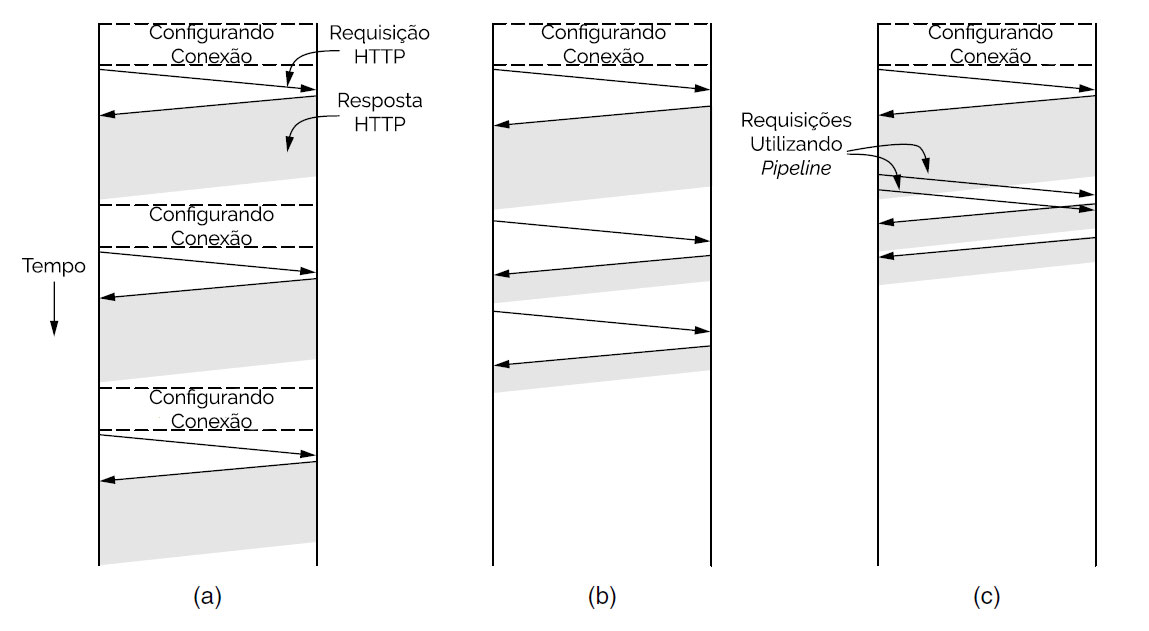
\includegraphics[width=1.0\textwidth]{./04-figuras/fund-teorica/httpconexaopersistente}
    \fonte{Adaptado de  \citeonline{Tanenbaum}}
    \label{fig:httpconexaopersistente}
\end{figure}

Uma funcionalidade desejada no HTTP/1.1 era a de poder fazer requisições para outros servidores além daquele da página principal sendo acessada. Dessa forma desenvolvedores podem hospedar arquivos CSS e JavaScript em um servidor e imagens em outro por exemplo. Isto se tornou possível com a adição da etiqueta \textit{Host}, com a qual o cliente pode definir qual é o caminho do servidor que será utilizado na requisição. Caso a etiqueta \textit{Host} não esteja definida no cabeçalho, é assumido que o caminho do servidor é o caminho da página principal.

Como concluem \citeonline{KeyDifferencesHTTP}: os protocolos HTTP/1.0 e HTTP/1.1 diferem em diversas maneiras. Enquanto muitas dessas mudanças têm o objetivo de melhorar o HTTP, a descrição do protocolo mais do que triplicou de tamanho, e muitas dessas funcionalidades foram introduzidas sem testes em ambientes reais. Esse aumento de complexidade causou muito trabalho para os desenvolvedores de clientes e servidores \textit{web}. 

No \autoref{qua:http11novo} encontra-se um resumo das mudanças introduzidos no protocolo HTTP/1.1.

\begin{quadro}[!htb]
	\centering
	\caption{Mudanças introduzidas no HTTP/1.1.
	\label{qua:http11novo}}
\end{quadro}
\begin{tabularx}{\textwidth}{| X | X |}
	\hline
	\multicolumn{2}{| c |}{\cellcolor[HTML]{C0C0C0}\textbf{Cabeçalhos}} \\
	\hline
	\textbf{Etiqueta} & \textbf{Descrição} \\
	\hline
	\textit{Accept-Encoding}\footnote{A etiqueta \textit{Accept-Encoding} já existia no HTTP/1.0, mas era pouco utilizada por causa da sua especificação confusa, por isso foi redefinida na versão 1.1.} & Lista de codificações aceitas. \\
	\hline
	\textit{Age} & O tempo que o conteúdo está salvo no \textit{proxy} em segundos. \\
	\hline
	\textit{Cache-Control} & Notifica todos os mecanismos de cache do cliente ao servidor se o conteúdo deve ser salvo. \\
	\hline
	\textit{Connection} & Controla a conexão atual. \\
	\hline
	\textit{Content-MD5} & Codificação binária de base-64 para verificar conteúdo da resposta. \\
	\hline
	\textit{ETag} & Identificador único de um conteúdo. \\
	\hline
	\textit{Host} & Indica o endereço e a porta do servidor que deve ser utilizado pela mensagem. \\
	\hline
	\textit{If-Match} & Realize a ação requisitada se, e somente se, o conteúdo do cliente é igual ao conteúdo do servidor. \\
	\hline
	\textit{If-None-Match} & Retorna código 304 se o conteúdo não foi modificado. \\
	\hline
	\textit{If-Range} & Se o conteúdo não foi modificado, envie a parte solicitada, se não, envie o conteúdo novo. \\
	\hline
	\textit{If-Unmodified-Since} & Envie o conteúdo se, e somente se, ele não foi modificado na data esperada. \\
	\hline
	\textit{Keep-Alive} & Detalhes sobre a conexão, tempo que ela ficará aberta e número máximo de requisições aceitas por ela. \\
	\hline
	\textit{Proxy-Authentication} & Pede uma,requisição de autenticação de um \textit{proxy}. \\
	\hline
	\textit{Proxy-Autorization} & Credenciais de autorização para se conectar a um \textit{proxy}. \\
	\hline
	\textit{Range} & Faz a requisição de apenas uma parte de um conteúdo. \\
	\hline
	\textit{Trailer} & Indica que o grupo de cabeçalhos está presente em uma mensagem. \\
	\hline
	\textit{Transfer-Encoding} & A forma de codificação usada para se transferir o conteúdo para o usuário. \\
	\hline
	\textit{Upgrade} & Pede para o servidor atualizar para outro protocolo. \\
	\hline
	\textit{Vary} & Informa quais partes do cabeçalho de requisição devem ser levadas em conta para descobrir se um recurso em \textit{cache} deve ser utilizado ou se este recurso deve ser solicitado no servidor. \\
	\hline
	\textit{Via} & Informa o servidor de \textit{proxies} pelos quais a requisição passou. \\
	\hline
	\textit{Warning} & Mensagem genérica de cuidado para possíveis problemas no corpo da mensagem. \\
	\hline
	\textit{WWW-Authenticate} & Indica tipo de autenticação que deve ser utilizada para acessar entidade requerida. \\
	\hline
	\multicolumn{2}{| c |}{\cellcolor[HTML]{C0C0C0}\textbf{Métodos}} \\
	\hline
	\textbf{Método} & \textbf{Descrição} \\
	\hline
	\textit{OPTIONS} & Solicita informações sobre os recursos que o servidor suporta. \\
	\hline
	\multicolumn{2}{| c |}{\cellcolor[HTML]{C0C0C0}\textbf{Estados}\footnote{Além dos citados ainda foram adicionados outros estados no HTTP/1.1, mas a lista ficaria muito extensa. Logo foram descritos os estados que podem influenciar no desempenho do \textit{front-end}.}} \\
	\hline
	\textbf{Código} & \textbf{Descrição} \\
	\hline
	100 & Confirma que o servidor recebeu o cabeçalho de requisição e que o cliente deve continuar a enviar a mensagem desejada. \\
	\hline
	206 & O servidor está entregando apenas uma parte de um conteúdo por causa da etiqueta de Range na requisição do cliente. \\
	\hline
	300 & Indica as multiplas opções disponíveis para o cliente. \\
	\hline
	409 & Indica que a requisição não pôde prosseguir por causa de um conflito. \\
	\hline
	410 & Indica que o conteúdo requisitado não está mais disponível e não estará disponível no futuro.\\
	\hline
	\multicolumn{2}{| c |}{\cellcolor[HTML]{C0C0C0}\textbf{Diretivas}} \\
	\hline
	\textbf{Diretiva} & \textbf{Descrição} \\
	\hline
	\textit{chuncked} & Utilizado para envio de conteúdo em partes. \\
	\hline
	\textit{max-age} & Determina qual é o tempo máximo que um conteúdo deve ficar salvo em \textit{cache}. \\
	\hline
	\textit{no-store} & Indica que o conteúdo não deve ser salvo em \textit{cache}. \\
	\hline
	\textit{no-transform} & Indica,que o conteúdo não deve ser modificado por \textit{proxies}. \\
	\hline
	\textit{private} & Indica que o conteúdo não deve ser acessado sem autenticação. \\
	\hline
	\multicolumn{2}{| c |}{\cellcolor[HTML]{C0C0C0}\textbf{Tipos de MIME}} \\
	\hline
	\textbf{Tipo} & \textbf{Descrição} \\
	\hline
	\textit{multipart/byteranges} & Indica que o conteúdo que está sendo enviado é apenas uma parte de um todo. \\
	\hline
	\multicolumn{2}{| c |}{\cellcolor[HTML]{C0C0C0}\textbf{Funcionalidades}} \\
	\hline
	\textbf{Nome} & \textbf{Descrição} \\
	\hline
	\textit{Content negotitation} & Escolhe a melhor representação disponível para um conteúdo. \\
	\hline
	\textit{Persistent connection} & Após o termino de uma requisição HTTP a conexão continua aberta e pode ser utilizada por outras requisições. \\
	\hline
	\textit{Pipeline} & O cliente não precisa esperar que a resposta de uma requisição retorne antes de enviar outra requisição. \\
	\hline
\end{tabularx}

\section{HTTP/1.1 VS HTTP/2}
\label{sec:http_11_vs_http_2}

O HTTP/1.1 é robusto e flexível, e isso permitiu que passasse a ser utilizado em aplicações diversas de maneira eficiente. Ao longo dos anos o IETF acrescentou algumas extensões ao protocolo para corrigir erros pontuais, mas o HTTP atendia as necessidades da rede mundial de computadores.

No inicio do século XXI, os \textit{websites} começaram a mudar. Eles se tornaram mais complexos e consequentemente maiores, muitas fontes e folhas de estilo eram utilizadas e cada página passou a possuir vários arquivos de JavaScript. Além disso, eles deixaram de ser estáticos e passaram a responder dinamicamente às ações dos usuários. Hoje em dia, muitas requisições HTTP são necessárias para se montar uma página \textit{web} e essas requisições podem ser longas e demoradas. Esse aumento da complexidade das páginas \textit{web} fez com que o HTTP/1.1 se tornasse um gargalo de desempenho para os \textit{websites}, então em 2007 o IETF formou o grupo HTTPbis (onde o "\textit{bis}" quer dizer "de novo" em latim). Mas o grupo só começou as discussões sobre a nova versão do protocolo em 2012, terminando de redigir as especificações em 2014. Após revisões, a especificação oficial da nova versão do HTTP foi aprovada no início do ano de 2015 e deve começar a ser utilizada em 2016. A nova versão do HTTP passou a se chamar HTTP/2. As casas decimais, que eram comuns na nomenclatura das outras versões, deixaram de existir, agora, caso mudanças sejam necessárias, serão lançadas novas versões do protocolo ao invés de sub-versões.

O HTTP/2 têm o objetivo de corrigir o problema de latência existente na versão anterior. Apesar do sistema de \textit{pipeline}, o HTTP/1.1 é muito sensível à latência, ou seja, apesar de conseguir uma grande quantidade de dados existem problemas quanto ao tempo de viagem das requisições e respostas. Isso acontece porque o \textit{pipeline} do HTTP/1.1 é muito difícil de ser gerenciado e muitas vezes fecha conexões que deveriam ter ficado abertas. O problema é tão grande que \citeonline{HTTP2Explained} afirma que, mesmo nos dias de hoje, muitos navegadores \textit{web} preferem desativar o \textit{pipeline}. Para corrigir este problema, o HTTP/2 propõe mudanças na forma como as informações são trocadas entre clientes e servidores. Assim como ocorreu na mudança da versão 1.0 para a versão 1.1, o novo protocolo não deve alterar nenhum paradigma já existente. As aplicações que utilizam o HTTP/1.1 devem continuar funcionando no HTTP/2, os formatos de arquivos, as URL e as URI devem ser mantidos e o usuário final não deve ter de fazer nada para poder aproveitar das melhorias do novo protocolo. Com isso, para tentar criar um protocolo que funcionasse no mundo real tanto quanto no teórico, o HTTPbis decidiu se inspirar no protocolo SPDY. O SPDY \cite{SPDY} é um protocolo para troca de dados entre clientes e servidores\textit{web}. Ele foi criado pela Google em 2010 como uma alternativa ao HTTP. O SPDY tem como objetivo aumentar a velocidade dos \textit{websites} e aplicações que o utilizam, melhorando o desempenho da \textit{web} como um todo. A escolha de basear o HTTP/2 neste protocolo, veio do fato dele já vir sendo utilizado por várias aplicações ao longo dos anos e ter se provado um conceito funcional e eficiente.

A primeira mudança no HTTP/2 está na forma como ele escreve suas requisições e respostas. Em suas versões anteriores, o protocolo optou por utilizar o formato ASCII para estruturar suas requisições e respostas, mas era difícil separar as partes dos cabeçalhos e tratar espaços em branco indesejados. Para resolver esse problema o HTTP/2 é um protocolo binário. Assim é mais simples quebrar requisições e respostas em quadros, compará-los e comprimir as informações. Entre as desvantagens dessa representação binária estão o fato de que os cabeçalhos HTTP não serão mais compreensíveis sem a ajuda de ferramentas de visualização de pacotes binários e que a depuração do protocolo dependerá de analisadores de pacotes.

Outro problema muito discutido entre os especialistas em desenvolvimento para a \textit{web} é a segurança da rede. Para garantir a proteção de seus usuário, alguns \textit{websites} e aplicações optam por utilizar serviços de rede seguro via TSL \footnote{http://pt.wikipedia.org/wiki/Transport\_Layer\_Security}. O TLS é um protocolo que promove a segurança entre as partes envolvidas em comunicações de dados através de autenticações e criptografias. Quando o HTTP é utilizado em conjunto com o TLS ele recebe o nome de HTTPS. Mas como explica \citeonline[p.~853]{Tanenbaum}, o HTTPS é simplesmente o protocolo HTTP, as diferenças estão no momento do transporte dos dados, quando o protocolo TLS realização ações para garantir a segurança. Foi muito discutida a ideia de fazer o uso do TLS obrigatório no HTTP/2, mas isto iria forçar todos os \textit{websites} e aplicações a se adaptarem para poderem se adequar ao protocolo. Então, ficou decidido que o uso do TLS continuaria opcional na nova versão.

Utilizando a representação binária, o HTTP/2 possibilita a multiplexação de fluxos de dados. Como explica \citeonline{HTTP2Explained}, uma fluxo é uma associação lógica criação por uma sequencia de quadros. No HTTP/2, uma conexão possui vários fluxos e por isso vários componentes podem ser transferidos ao mesmo tempo. Para esse processo funcionar o protocolo multiplexa esses fluxos no momento do envio e as separa novamente na chegada. A \autoref{fig:streamsmultiplexadas} ilustra a multiplexação de fluxos.

\begin{figure}[!htb]
    \centering
    \caption{Multiplexação de fluxos no HTTP/2 (a) dois fluxos separadas (b) fluxos multiplexadas}
    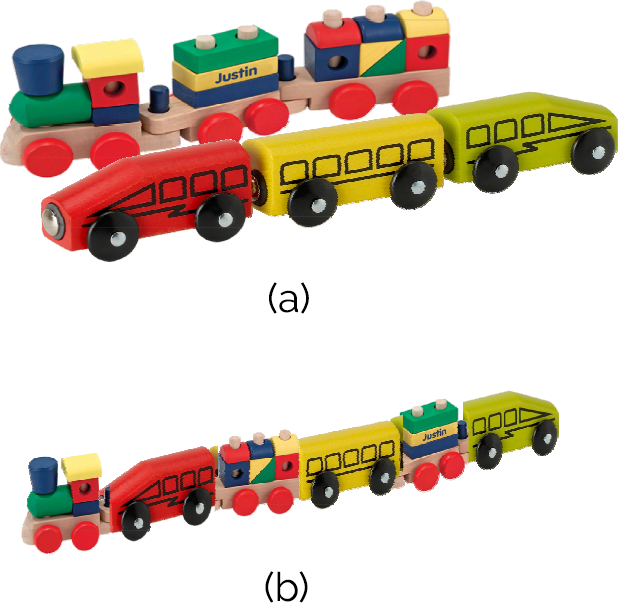
\includegraphics[width=0.5\textwidth]{./04-figuras/fund-teorica/multiplexed_streams}
    \fonte{Adaptado de  \citeonline{HTTP2Explained}}
    \label{fig:streamsmultiplexadas}
\end{figure}

Um problema no HTTP/1.1 era a garantia de que um componente A já teria sido baixado quando outro componente B que depende de A fosse executado. Apesar de o HTML garantir isso, essa limitação impedia que a paralelização de \textit{downloads} fosse maior. No HTTP/2 foram adicionados os mecanismos de prioridade e dependência. Eles tornaram possível indicar quais fluxos devem ser baixados primeiro e quais são suas interdependências. Dessa forma, os desenvolvedores de páginas \textit{web} podem paralelizar ao máximo seus componentes e o protocolo cuidará de evitar erros. 

A compressão de dados é um fator importante para o aumento de desempenho do HTTP. Com o passar dos anos, as requisições e respostas aumentaram de tamanho, e os algoritmos de compressão existentes para o SPDY e o HTTPS não se provaram eficientes contra ataques de terceiros. Logo notou-se que este era um ponto crítico para a nova versão do protocolo, então o HTTPbis decidiu por criar o HPACK, que será o novo formato de compressão para cabeçalhos HTTP/2. Visando a robustez desse formato, foi criada uma nova especificação exclusiva para o HPACK, que detalha como ele funciona e como deve ser usado \cite{HPACKSpec}.

Assim como na versão anterior, o HTTP/2 possui mecanismos para lidar com a \textit{cache}. As etiquetas existentes no HTTP/1.1 continuam a existir, mas uma nova funcionalidade foi adicionada na nova versão, o \textit{Server Push}. O \textit{Server Push} tem o objetivo de permitir que o cliente consiga componentes da maneira rápida, mesmo que seja a primeira vez que ele requisite aquele componente. A \textit{Server Push} funciona da seguinte maneira: o cliente requisita um componente X. O servidor então sabe que é provável que este mesmo cliente vá requisitar o componente Y nos próximos instantes. Sendo assim o servidor pode enviar o componente Y antes mesmo de receber o pedido por ele. Essa funcionalidade é algo que o cliente deverá especificar explicitamente, mas existe grande expectativa quanto às melhorias que ela pode trazer. Além dessa melhoria no sistema de \textit{cache}, o HTTP/2 inclui uma nova etiqueta para impedir o desperdício de banda de transmissão. Se o servidor começar a enviar um componente com um tamanho específico e perceber que aquele componente não é mais útil, ele pode cancelar o envio com a etiqueta \textit{RST STREAM}, evitando que o fluxo de envio fique ocupado com dados desnecessários por muito tempo.

Caso um \textit{website} ou uma aplicação deseje transferir o cliente para outro servidor sem ser o requisitado, ou até mesmo para outra porta, ele poderá utilizar a etiqueta Alt-Svc. Com essa etiqueta o servidor informa ao cliente para onde ele deve ir, então o cliente deve tentar se conectar de maneira assíncrona no caminho sugerido pelo Alt-Svc e utilizar aquela conexão apenas se ela se provar confiável. Essa etiqueta foi criada com a intensão de informar clientes que os dados requisitados estão disponíveis também em um servidor seguro.

A escolha pela utilização de envio através de fluxos, tem o objetivo de aumentar a velocidade do protocolo e a quantidade de dados que pode ser enviada de uma só vez. Cada um desses fluxos possui sua própria janela de envio independente, o que garantirá que se um fluxo falhe os outros continuem funcionando. Para impedir o envia de dados e parar todos os fluxos abertos, o protocolo inclui a etiqueta \textit{BLOCKED}, que informa que existem dados para serem enviados, mas algo está impedindo o processo de continuar.

O protocolo HTTP/2 traz grandes mudanças na estrutura dos dados que serão enviados e recebidos. A essência continua a mesma, um protocolo de requisições e respostas, mas, a medida que o protocolo evolui, novas formas de aprimoramento do desempenhos dos \textit{websites} e das aplicações estão sendo acrescentadas ao HTTP

O documento completo com toda a especificação do HTTP/2 pode ser encontrado em \cite{HTTP2Spec}. O \autoref{qua:http2novo} mostra um resumo das mudanças detalhadas anteriormente.

\begin{quadro}[!htb]
	\centering
	\caption{Mudanças introduzidas no HTTP/2. \label{qua:http2novo}}
	\begin{tabularx}{\textwidth}{| X | X |}
		\hline
		\textbf{Funcionalidade} & \textbf{Descrição} \\
		\hline
		HTTP/2 binário & Ao invés de utilizar caracteres ASCII para representar informações, o HTTP/2 é binário, o que facilita a comparação de informações, o envio de dados e outras funcionalidades. \\
		\hline
		Fluxos multiplexados & Se existem dois componentes para serem enviados, o protocolo pode optar por multiplexa-los em uma única stream e enviar os dois ao mesmo tempo. \\
		\hline
		Prioridades e dependencias & Caso existam, o cliente pode definir quais componentes possuem prioridade para serem baixados primeiro. Além disso pode informar se existem dependencias entre os  componentes para garantir que quando um arquivo seja baixado todos os outros necessários para o seu funcionamento já estejam no cliente. \\
		\hline
		\textit{HPACK} & Novo sistema de compressão de cabeçalhos para o HTTP/2. \\
		\hline
		RST\_STREAM & Uma maneira de cancelar o envio de componentes. \\
		\hline
		\textit{Server Push} & Habilidade do servidor de enviar um arquivo X para o cliente caso ele veja como provável que o cliente vai precisar desse arquivo no futuro próximo. \\
		\hline
		Janelas individuais de fluxo & Cada fluxo de envio possui sua própria janela que pode ser gerenciada individualmente, assim caso um fluxo falhe os outros continuam. \\
		\hline
		\textit{BLOCKED} & Forma do cliente ou servidor informar a outra parte que existe algo impedindo que o envio de dados continue. \\
		\hline
		Alt-Svc & O servidor pode informa ao cliente de caminhos alternativos para acessar os dados requisitados. \\
		\hline
	\end{tabularx}
\end{quadro}

\newpage
\section{AJAX}
\label{sec:ajax}
AJAX é a sigla em inglês para "Assíncrono JavaScript + XML", e foi inventada por \citeonline{AJAX}. Mas isso não quer dizer que Garrett tenha inventado o modelo AJAX utilizado pelos \textit{websites} e aplicações.

Como dito pelo próprio \citeonline{AJAX}, "AJAX não é uma tecnologia". Na realidade AJAX é a definição de como várias tecnologias podem ser utilizadas em conjunto para ler componentes \textit{web} de maneira assíncrona. Estas tecnologias incluem:
	\begin{itemize}
		\item HTML ou XHTML\footnote{http://en.wikipedia.org/wiki/XHTML}
		\item CSS
		\item JavaScript
		\item DOM\footnote{http://www.w3.org/DOM/}
		\item XML e XSLT\footnote{http://www.w3schools.com/xml/, http://www.w3schools.com/xsl/}
		\item Requisições XMLHttp (\textit{XMLHttpRequest})\footnote{https://developer.mozilla.org/en-US/docs/Web/API/XMLHttpRequest}
	\end{itemize}

A \autoref{fig:compajax} mostra uma comparação entre o modelo clássico de chamadas \textit{web} e o modelo utilizando AJAX. O modelo AJAX adiciona uma camada intermediária entre o usuário e o servidor.

Quando o usuário interage com a página \textit{web} ele manda uma mensagem para essa nova camada, desenvolvida em JavaScript, que é responsável por requisitar do servidor somente os dados necessários para a interação do usuário e atualizar apenas a parte da página necessária para terminar essa interação. Dessa forma o AJAX impede que as páginas tenham de ser inteiramente recarregadas a cada interação e consegue melhorar a experiência do usuário.

\begin{figure}[!htb]
    \centering
    \caption{Comparação entre modelo de \textit{web} original e modelo utilizando AJAX}
    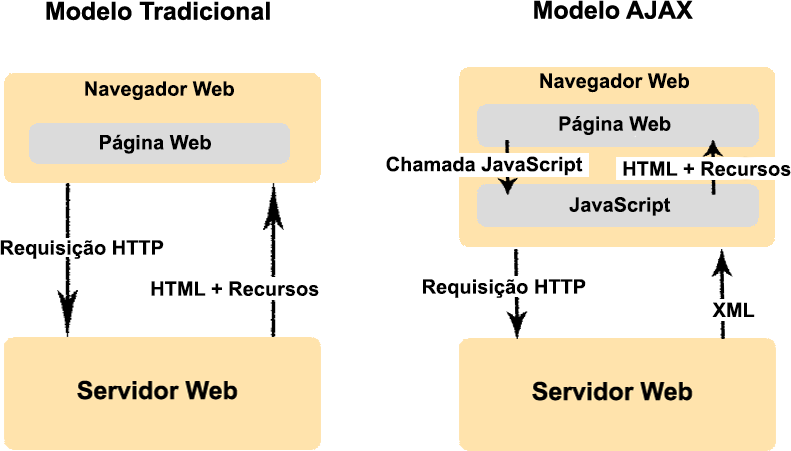
\includegraphics[width=0.7\textwidth]{./04-figuras/fund-teorica/comparacao_ajax}
    \fonte{Adaptado de \citeonline{FigAjax}}
    \label{fig:compajax}
\end{figure}


\section{Web 2.0}
\label{sec:web20}
A \textit{Web} 2.0 não é uma nova versão da \textit{World Wide Web} criada por Tim Berners-Lee. Como explica \citeonline{Web20}, o termo \textit{Web} 2.0 surgiu de uma discussão entre a companhia de mídia O'Reilly e a empresa de produção de MediaLive, quando estavam preparando uma conferencia sobre a \textit{web}. O que eles chamaram de \textit{Web} 2.0 foi a nova forma como a criação de Berners-Lee estava sendo utilizada pelas pessoas.

O desenvolvimento de técnicas AJAX e o conceito de conhecimento coletivo fez com que a \textit{web} deixasse de ser utilizada apenas para mostrar páginas estáticas e passasse a explorar a interação com o usuário. Sendo assim \textit{websites} se tornaram aplicações \textit{web}, que melhoravam a medida que os usuários iam alimentando-as com novas informações. Como exemplo de aplicações que exploram os conceitos definidos na \textit{Web} 2.0 podemos citar a Wikipedia \footnote{https://www.wikipedia.org/}, o Facebook \footnote{https://www.facebook.com/} e o Google Maps \footnote{https://www.maps.google.com/}. Todas essas aplicações utilizam de técnicas AJAX para garantir uma boa experiência e são alimentadas com informações entradas pelos usuários, o que as torna mais dinâmicas e flexíveis do que os \textit{websites} da \textit{Web} 1.0 (como ficou conhecida a primeira fase da \textit{web}).